\documentclass[a4paper,11pt]{article}

\usepackage[T1]{fontenc}
\usepackage[polish]{babel}
\usepackage[utf8]{inputenc}
\usepackage{lmodern}
\selectlanguage{polish}
\usepackage[top=2cm, bottom=2cm, left=1cm, right=1cm]{geometry}
\makeatletter
\newcommand{\linia}{\rule{\linewidth}{0.4mm}}
\renewcommand{\maketitle}{\begin{titlepage}
    \vspace*{2cm}
    \begin{center}\LARGE
    Politechnika Warszawska\\
    Wydział Elektryczny\\
    \end{center}
    \vspace{5cm}
    \noindent\linia
    \begin{center}
      \LARGE \textsc{\@title}
         \end{center}
     \linia
    \vspace{0.5cm}
    \begin{flushright}
    \begin{minipage}{5cm}
    \textit{Autor:}\\
    \normalsize \textsc{\@author} \par
    \end{minipage}
    \vspace{5cm}
     \end{flushright}
    \vspace*{\stretch{6}}
    \begin{center}
    \@date
    \end{center}
  \end{titlepage}
}
\makeatother
\author{Grzegorz Kopyt}
\title{Specyfikacja Funkcjonalna \\
,,Arbitrage''}
\usepackage{graphicx}

\begin{document}

\maketitle

\tableofcontents
\vspace{1cm}
\noindent\linia
\section{Wstęp teoretyczny}
Podstawą programu jest analiza podanych kursów walut, pod kątem korzyści z zakupu i sprzedaży.

Jednym z zadań jest znalezienie takiej serii wymian waluty wyjściowej, aby jak najkorzystniej dokonać zakupu innej waluty.

Drugim zadaniem jest wskazanie takiej serii wymiany walut, aby ostatecznie otrzymać większą kwotę w walucie wyjściowej niż początkowa, którą dysponował użytkownik.

Wymiany walut mogą być obarczone opłatą stała lub procentową (od kwoty docelowej).

\noindent\linia
\section{Wymagania funkcjonalne}
\begin{itemize}
\item Podanie przez użytkownika pliku z kursami walut (w narzuconym przez nas formacie).
\item Podanie informacji o tym jaką walutą użytkownik dysponuję  i jaką chce kupić. (Korzystny zakup waluty)
\item Podanie kwoty wyjściowej (bez waluty) jaką użytkownik dysponuje. (Zwiększenie kwoty jaką dysponujemy)
\item Odczytanie wyników z okna aplikacji.
\end{itemize}

\noindent\linia
\section{Obsługa}

\begin{center}
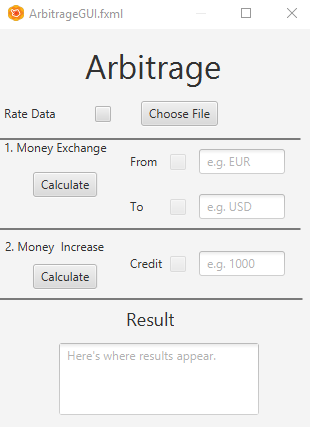
\includegraphics[scale=1]{ArbitrageGUI}
\end{center}

\begin{itemize}
\item \textbf{Podanie pliku z kursami walut:}
\begin{enumerate}
\item Naciśnij przycisk \textit{Choose file} - pojawi się okno wyboru pliku z twojego systemu.
\item Wybierz plik i zatwierdź - powrócisz do ekranu początkowego.
\item W kwadracie obok przycisku \textit{Choose file} pojawi się znaczek, potwierdzający dokonanie operacji wyboru pliku.


\includegraphics[width=5cm]{FileChosen}
\end{enumerate}

\item  \textbf{Korzystna wymiana waluty:}
\begin{enumerate}
\item W pierwszej sekcji (\textit{Money Exchange}) w pole tekstowe na prawo od napisu \textit{From} należy podać skróconą nazwę waluty, za którą chcemy dokonać zakupu.
\\ Po tej operacji w kwadracie po lewej stronie pola tekstowego pojawi się znaczek potwierdzający podanie skróconej nazwy waluty.
\item Poniżej, w pole tekstowe na prawo od napisu \textit{To} należy wpisać skróconą nazwę waluty, której zakupu chcemy dokonać.
\\ Po tej operacji w kwadracie po lewej stronie pola tekstowego pojawi się znaczek potwierdzający podanie skróconej nazwy waluty.
\item Następnie należy wcisnąć przycisk \textit{Calculate} znajdujący się w sekcji \textit{Money Exchange}.
\item Wynik operacji pojawi się w polu tekstowym pod napisem \textit{Result}.
\end{enumerate}
\textit{UWAGA! Należy operować na skróconych nazwach podanych w pliku z kursami walut. Wielkość liter ma znaczenie.}
\newpage
\item  \textbf{Zarabianie na wymianie walut:}
\begin{enumerate}
\item W drugiej sekcji (\textit{Money Increase}) w pole tekstowe na prawo od napisu \textit{Credit} należy podać kwotę, którą dysponujemy.
\item Następnie należy wcisnąć przycisk \textit{Calculate} znajdujący się w sekcji \textit{Money Increase}.
\item Wynik operacji pojawi się w polu tekstowym pod napisem \textit{Result}.
\end{enumerate}
\item\textbf{ Wyniki}
\begin{itemize}
\item Przejścia między walutami (ścieżki) będą przedstawione w taki sposób: \emph{EUR->USD->PLN}
\\Oznacza to, że euro wymieniliśmy na amerykańskie dolary, a dolary na złotówki.
\item W przypadku operacji z sekcji \textit{Money Increase} w ostatniej linii wyniku wyświetlona zostanie spodziewana kwota końcowa.
\end{itemize}
\end{itemize}

\noindent\linia
\section{Komunikaty o błędach}
W przypadku wystąpienia błędu wyskoczy okno z informacją o błędzie.
\begin{itemize}
\item Błędny plik wejściowy. (pojawi się informacja o tym, w której linii pliku pojawiła się niezgodność z wzorem)
\item Pola tekstowe będą przystosowane do wpisywania tylko pożądanych wartości. Wpisanie wartości nieprawidłowej będzie niemożliwe.
\item W przypadku kiedy użytkownik nie wypełnił wszystkich potrzebnych pól, a nacisnął przycisk \textit{Calculate} pojawi się prośba o uzupełnienie pozostałych potrzebnych pól.
\end{itemize}

\noindent\linia
\section{Testy akceptacyjne}

\begin{itemize}
\item 

\end{itemize}

\noindent\linia

\end{document}



